\subsubsection{Ameaça à Infraestrutura Crítica: Setor Elétrico e Saúde (SUS)}

A integração central do projeto foi materializada na intersecção veloz entre as medições dos satélites termais e a infraestrutura civil mapeada. Centros hospitalares localizados nos arredores dos epicentros rurais de incêndio sofreram o reflexo primário de densas massas regionais de fumaça, gerando alto impacto na região de cobertura das unidades de saúde. O controle exibido na Figura \ref{fig:hospitais_criticos} rastreou não apenas o quantitativo, mas a intensidade da radiação (FRP) sobrepostas às coordenadas do Cadastro Nacional de Estabelecimentos de Saúde (CNES).

\begin{figure}[H]
    \centering
    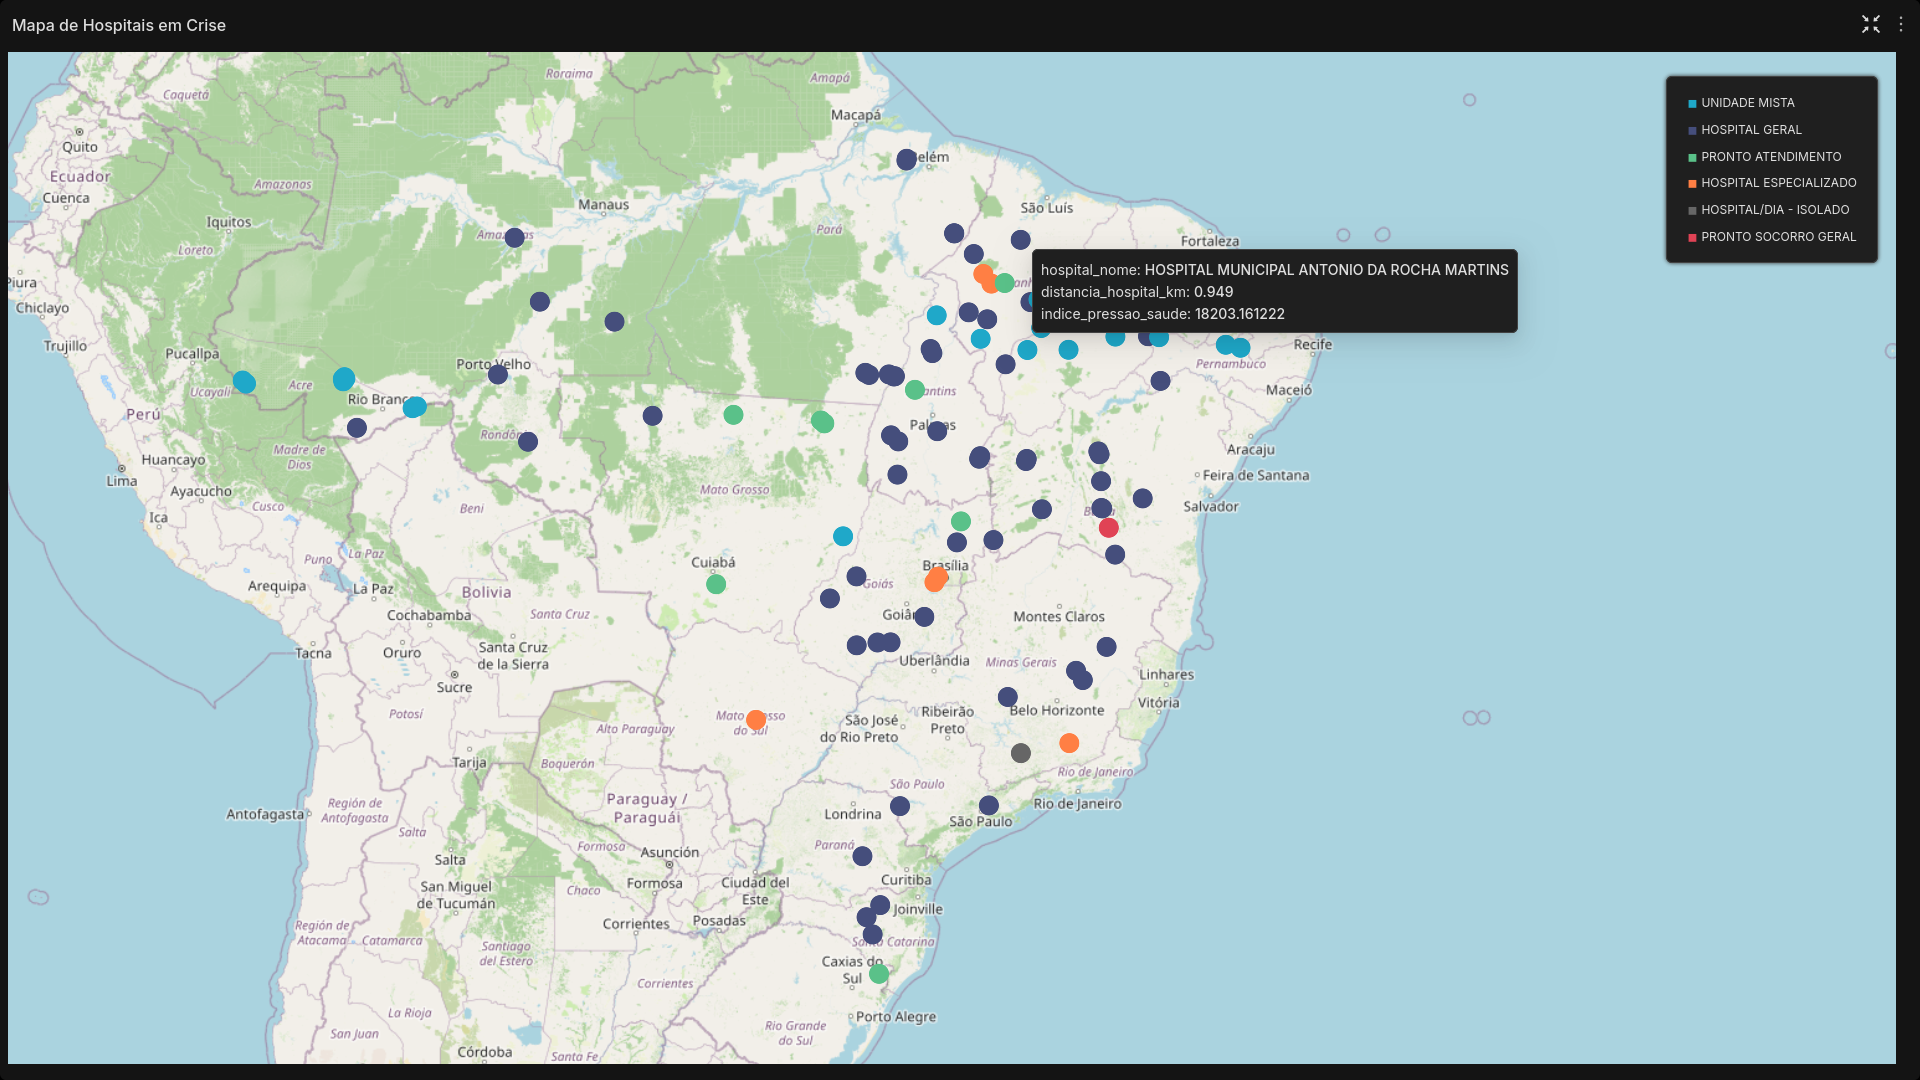
\includegraphics[width=0.9\textwidth]{materiais_apoio/figures/HospitaisCriticos.png}
    \caption{Monitoramento de Hospitais Expostos ao Fogo.}
    \label{fig:hospitais_criticos}
\end{figure}

Da mesma forma sistêmica, os dados estenderam o cordão sanitário para resguardar a malha operada pelo Operador Nacional do Sistema Elétrico (ONS). A exposição das linhas de transmissão a focos de calor intenso gera o perigo extremo de arcos elétricos e curtos-circuitos da rede neutra para a terra (desligamento forçado). 

A Figura \ref{fig:evolucao_energia} modela a progressão sistêmica dessa ameaça ao longo de todo o ano de 2025. A série temporal atua como uma evidência analítica crucial para demonstrar a assimetria da crise: o índice permanece baixo no primeiro semestre e cresce de forma acentuada a partir de setembro e outubro nas regiões de escoamento energético. Essa métrica expõe como as condições de seca extrema submetem repentinamente a infraestrutura a um aumento de pressão crítico e de complexa mitigação logística.

\begin{figure}[H]
    \centering
    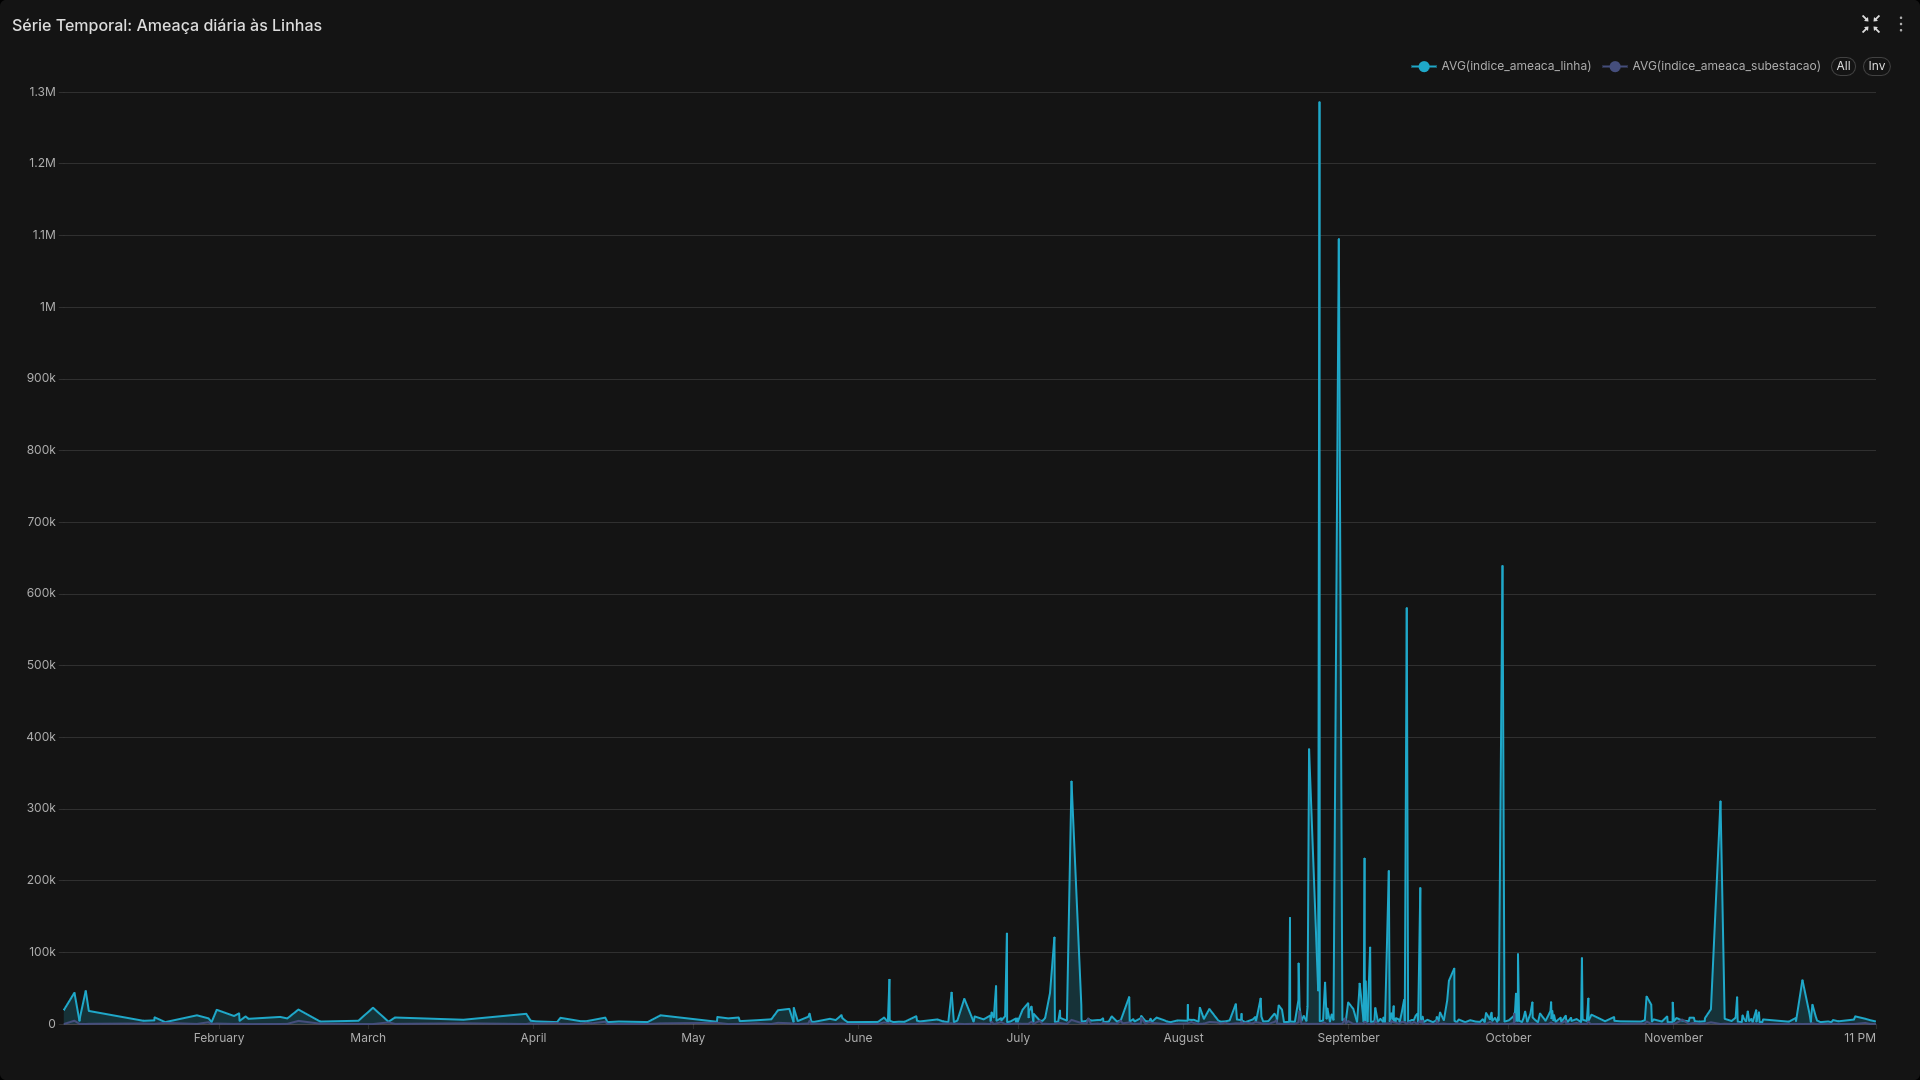
\includegraphics[width=0.9\textwidth]{materiais_apoio/figures/EvoluçãoDaPressãoEletricaAolongodoAno.png}
    \caption{Evolução da Ameaça à Infraestrutura Elétrica (ONS).}
    \label{fig:evolucao_energia}
\end{figure}

Aliando o risco termal agudo com as métricas topológicas (\textit{Betweenness Centrality}) previamente estabelecidas, a plataforma consolidou a Tabela \ref{tab:subestacoes_ameacadas}. Ela enumera as subestações mais expostas a interrupções operacionais, ordenadas pelo potencial de indução de risco sistêmico em rede. O cruzamento destacou vértices infraestruturais vitais, a exemplo da SE Rio Verde Norte (GO), elo de escoamento do Norte para o Sudeste; da SE Assis (SP), coletora da bacia do Rio Paraná; e da SE Trindade (GO), pivô na interligação Norte-Sul \cite{epe_pde_2032, ons_mapa_2026}.

Quando nós de energia sob Risco \textbf{Extremo} sofrem desligamento forçado, a matriz energética redistribui a carga base por rotas mais longas. Esse fenômeno sobrecarrega linhas secundárias e aciona sistemas primários de proteção (como o Esquema Regional de Alívio de Carga - ERAC), culminando no risco agudo de apagões regionais e blecautes em cascata por todo o subsistema interligado do país \cite{ons_procedimentos_2026}.

\begin{table}[H]
\centering
\caption{Top 10 Subestações Críticas via Betweenness Centrality.}
\label{tab:subestacoes_ameacadas}
\resizebox{\textwidth}{!}{%
\begin{tabular}{lrrc}
\toprule
\textbf{Subestação} & \textbf{Capacidade (MW)} & \textbf{Betweenness Centrality} & \textbf{Risco Cascata} \\
\midrule
R.VERDE NORTE & 1344.00 & 100.00 & EXTREMO \\
ASSIS & 2808.00 & 98.21 & EXTREMO \\
TRINDADE & 1600.00 & 91.33 & EXTREMO \\
SAMAMBAIA & 6000.00 & 89.30 & EXTREMO \\
XAVANTES & 600.00 & 89.22 & EXTREMO \\
BANDEIRANTES & 2542.00 & 87.68 & EXTREMO \\
LONDRINA ESU & 2016.00 & 59.42 & ALTO \\
BOM.JES.LAPA II & 850.00 & 47.07 & MEDIO \\
LUZIANIA & 450.00 & 46.83 & MEDIO \\
MIRACEMA & 10359.00 & 45.51 & MEDIO \\
\bottomrule
\end{tabular}%
}
\end{table}

